\subsection{Mechanism: Semantic Feedback IR (E6)}
Table~\ref{tab:e6-conf} holds $K$ and task count fixed and sweeps feedback
content. Full Semantic IR (variant~C) improves mean conformance by
\textbf{+7.7\,pp} over test-only (A)---the paper's lead empirical claim.

\begin{table}[t]
  \centering
  \caption{E6 feedback variants ($n{=}120$, $K{=}3$).}
  \label{tab:e6-conf}
  \footnotesize
  \begin{tabular}{lcc}
    \toprule
    Variant & Feedback & Conf.\ (\%) \\
    \midrule
    A & test only       & 79.1 \\
    B & test + expected & 78.9 \\
    C & full Semantic IR & \textbf{86.9} \\
    \bottomrule
  \end{tabular}
\end{table}

\subsection{Overlap evidence (E3 + E10)}
Figure~\ref{fig:overlap} and Table~\ref{tab:deploy} synthesise E3/E10.
Canonical E3 tertiles are \emph{non-monotone} (M does not uniformly beat B2).
On unfiltered random tasks (E10), B2 reaches 89.1\% vs.\ M 83.1\% (0/100 wins).

\begin{figure}[t]
  \centering
  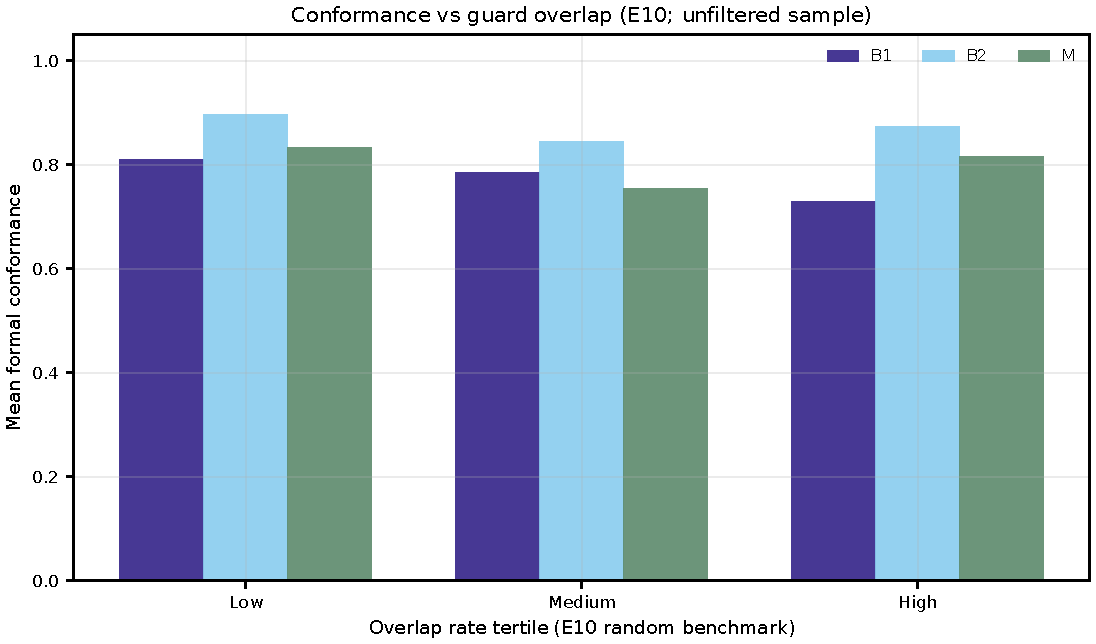
\includegraphics[width=\linewidth]{../hsp-agile/figures/performance_vs_overlap.pdf}
  \caption{E10 conformance vs.\ overlap-rate tertile (B1/B2/M).}
  \label{fig:overlap}
\end{figure}

\begin{table}[t]
  \centering
  \caption{Deployment boundary: when to prefer B2 vs.\ full M.}
  \label{tab:deploy}
  \footnotesize
  \begin{tabular}{@{}p{0.22\linewidth}p{0.34\linewidth}p{0.34\linewidth}@{}}
    \toprule
    \textbf{Signal} & \textbf{Prefer B2} & \textbf{Prefer M} \\
    \midrule
    Overlap / sampling & E10, E12 aggregate & E6 typed IR (+7.7\,pp) \\
    Release bar & Mean Conf.\ sufficient & Conjunctive $\mathrm{Accept}$ \\
    Prevention & --- & PDR 95\% / FAR 5\% (E2) \\
  \end{tabular}
\end{table}

\subsection{Prevention (E2)}
Under conjunctive Accept, strict success is uniformly low (5\% across modes).
M improves prevention: PDR 95.0\%, FAR 5.0\% vs.\ B2 91.2\%/8.8\%---the
operational reason to deploy full M despite higher latency ($3.3\times$ B2).

\subsection{Aggregate effectiveness (E1, footnote)}
Canonical E1 (seed~0): B1 89.2\%, B2 87.7\%, M 86.3\%---all Holm n.s.
E12-canonical ($120{\times}3$ seeds): B2 leads every seed (88.0\% mean vs.\
M 86.0\%); M wins 4/120 paired comparisons; Friedman $p{=}0.077$.
